\documentclass[12pt,a4paper]{article}
\usepackage{amsmath}
\usepackage{mathtext}
\usepackage{icomma}
\usepackage{amsfonts}
\usepackage{amssymb}
\usepackage[utf8]{inputenc}
\usepackage[T1,T2A]{fontenc}
\usepackage[english, russian]{babel}
\usepackage{graphicx}
\usepackage[left=2cm,right=2cm,top=2cm,bottom=2cm]{geometry}
\usepackage{calc}
\usepackage{wrapfig}
\usepackage{setspace}
\usepackage{indentfirst}
\usepackage{subfigure}
\usepackage[table,xcdraw]{xcolor}
\usepackage{float}

\title{Отчет о выполнении лабораторной работы 3.4.2\\
Закон Кюри-Вейсса}

\author{Исламов Сардор, группа Б02-111}
\date{26 ноября 2022 г.}

\begin{document}
\maketitle
\subparagraph*{Аннотация.} 
В работе исследована зависимость периода колебаний автогенератора от температуры сердечника катушки.
По результатам измерений определена парамагнитная точка Кюри гадолиния.

\subsection*{Теоретическое введение}
Вещества с отличными от нуля атомными магнитными моментами обладают парамагнитными свойствами. 
Внешнее магнитное поле ориентирует магнитные моменты, которые в отсутствие поля располагались в пространстве хаотическим образом. 
Однако при $T \rightarrow 0$ тепловое движение всё меньше препятствует магнитным моментам атомов ориентироваться в одном направлении при сколь угодно слабом внешнем поле. 
В ферромагнетиках -- под влиянием обменных сил -- это происходит при понижении температуры не до абсолютного нуля, а до температуры Кюри $\Theta$. 
Оказывается, что у ферромагнетиков магнитная восприимчивость должна удовлетворять закону Кюри-Вейсса:
\begin{equation}
    \label{eq:Kuri-Veicca}
    \chi \propto \frac{1}{T-\Theta_p},
\end{equation}
где $\Theta_p$ -- температура, близкая к температуре Кюри, так как при $T \approx \Theta$ формула~(\ref{eq:Kuri-Veicca}) недостаточна точна.

\subsection*{Экспериментальная установка}
Схема установки для проверки закона Кюри-Вейсса показана на рис.~\ref{ris:ustanovka}. Исследуемый ферромагнитный образец (гадолиний) расположен внутри пустотелой катушки самоиндукции, которая служит индуктивностью колебательного контура, входящего в состав LC-автогенератора. 
Автогенератор собран на полевом транзисторе КП-103 и смонитрован в виде отдельного блока.
\begin{figure}[H]
    \centering
    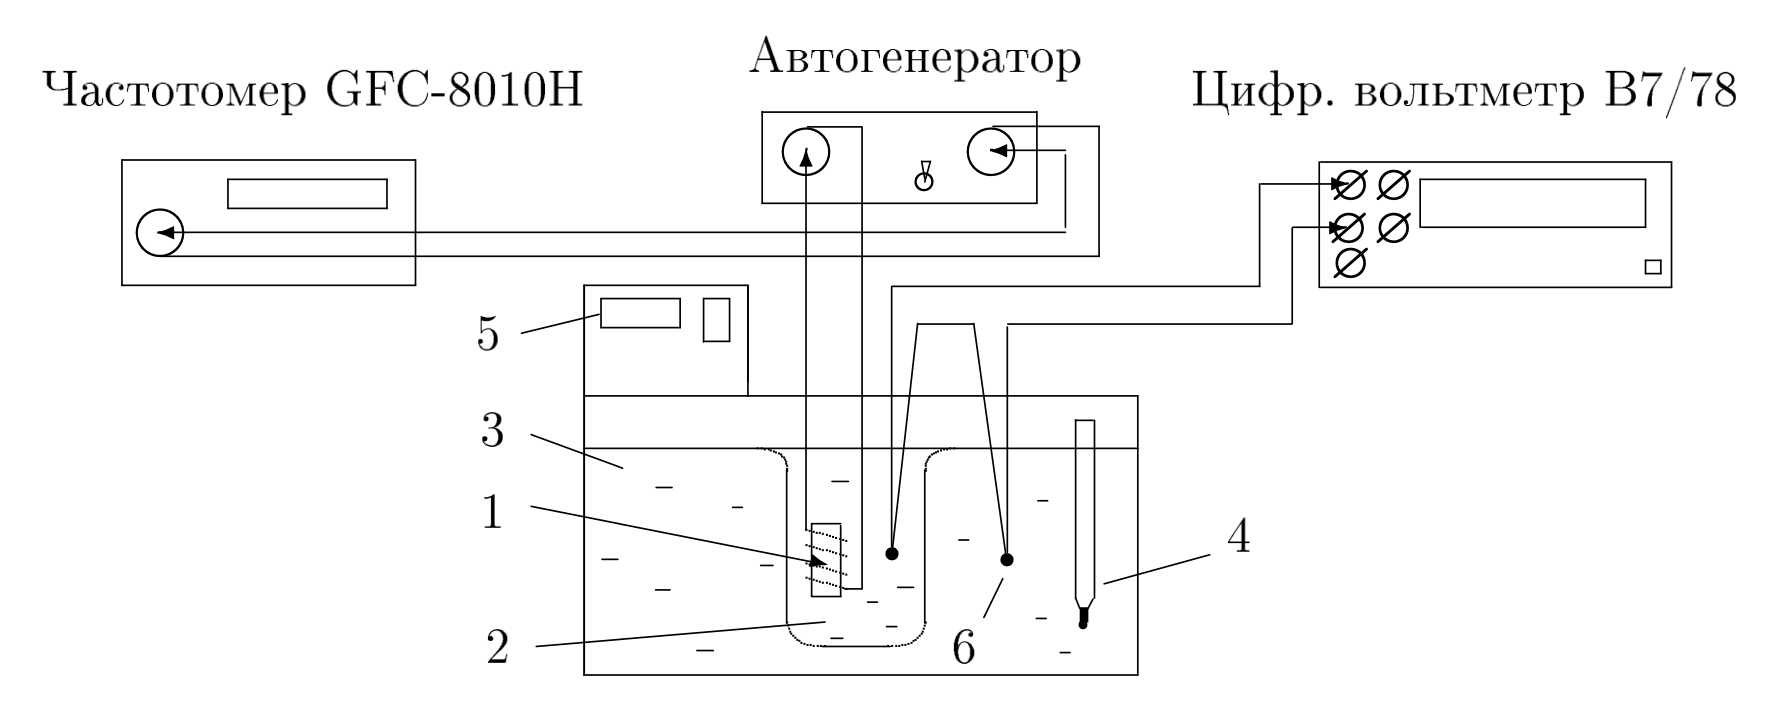
\includegraphics[width=0.7\linewidth]{pics/scheme.png}
    \caption{Схема экспериментальной установки.}
    \label{ris:ustanovka}
\end{figure}

Магнитная воосприимчивость образца $\chi$ определяется по изменению самоиндукции катушки. 
Обозначив через $L$ самоиндукцию катушки с образцом и через $L_0$ -- её самоиндукцию в отсутствие образца, получим
\[
    (L-L_0)\propto \chi.
\]

При изменении самоиндукции образца меняется период колебаний автогенератора:
\[    \tau = 2\pi \sqrt{LC}, \]
где $C$ -- ёмкость конутра автогенератора. Период колебаний в отсуствие образца опредлеяется самоиндукцией пустой катушки:
\[    \tau_0 = 2\pi \sqrt{L_0C}. \]

Итак, закон Кюри-Вейсса справедлив, если выполнено соотношение:
\begin{equation}
    \frac{1}{\chi} \propto (T-\Theta_p) \propto \frac{1}{\tau^2-\tau_0^2}
\end{equation}

\subsection*{Результаты измерений и обработка данных}
Оценим допустимую ЭДС термопары: $\varepsilon = \Delta T / \kappa  \approx 0.02\ мВ$. 
Будем придерживаться данного значения, чтобы погрешности были не слишком большими.

Теперь исследуем зависимость периода колебаний $LC-$генератора от температуры образца (табл. 1).
Обозначим за $\tau$ период колебаний, измеренный по частотомеру, $T -$ температура, снятая с дисплея и $\Delta U-$ ЭДС термопары.
Также период колебаний без образца, указанный на установке, равен $\tau_0 = 6.9092\ с$.

\begin{table}[H]
    \centering
    \begin{tabular}{|c|c|c|c|}
    \hline
    $Т,  ^oC$ & $\Delta U$, -0.1 мкВ & $\tau_0$, мкс & $T, ^oC$ (с термостата) \\ \hline
    12        & 81                   & 8.0144036     & 12.14                   \\ \hline
    14        & 120                  & 7.9785881     & 14.12                   \\ \hline
    16        & 160                  & 7.9186441     & 16.11                   \\ \hline
    18        & 140                  & 7.8077556     & 18.10                   \\ \hline
    20        & 180                  & 7.6406484     & 20.10                   \\ \hline
    22        & 170                  & 7.4240262     & 22.09                   \\ \hline
    24        & 180                  & 7.2517720     & 24.10                   \\ \hline
    26        & 150                  & 7.1755204     & 26.10                   \\ \hline
    28        & 110                  & 7.1325068     & 28.10                   \\ \hline
    30        & 190                  & 7.1085357     & 30.09                   \\ \hline
    32        & 190                  & 7.0896154     & 32.08                   \\ \hline
    34        & 160                  & 7.0756342     & 34.09                   \\ \hline
    36        & 160                  & 7.0655102     & 36.09                   \\ \hline
    38        & 160                  & 7.0575413     & 38.08                   \\ \hline
    40        & 160                  & 7.0513568     & 40.08                   \\ \hline
    \end{tabular}
    \caption{Зависимость периода колебаний от температуры образца}
\end{table}

С учетом того, что $\Delta T = \kappa \Delta U$ - разность температур жидкости и образца (при $\Delta U > 0$ температура образца выше) изобразим зависимости на графике (рис. 2) и с использованием формулы (2) определим некторые характеристики образца.

\begin{figure}[H]
    \centering
    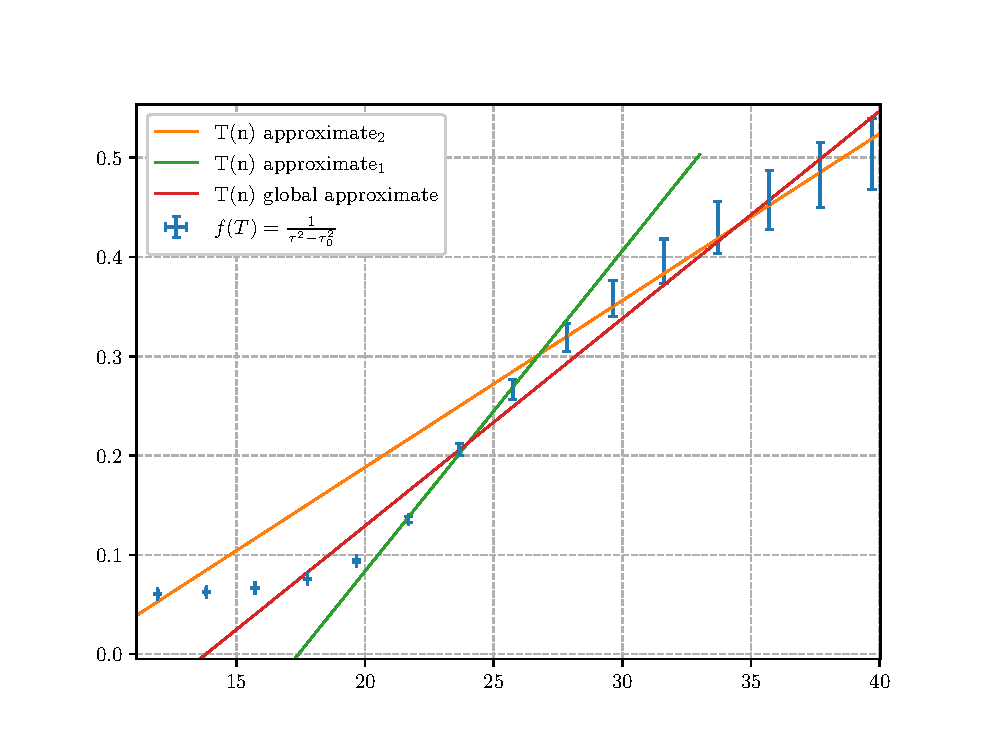
\includegraphics[width=\linewidth]{pics/ft.eps}
    \caption{зависимость периода колебаний от температуры образца}
\end{figure}

Как видно, участок кривой после изгиба не сразу выходит на прямую, что сильно сказывается на результатах.
Поэтому отдельно проводился анализ первого участка, второго, и зависимости в общем.
Наиболее соответствует табличным значениям зависимость сразу после изгиба (зеленая прямая), при этом точка Кюри равна соответственно $\theta = 17.42 \pm 1.67 ^oC$, для красной прямой при этом значение оказалось меньше 14, а для оранжевой меньше 9.
Табличное значение $\theta = 16^oC$.
\subsection*{Подведение итогов}
В ходе работы была исследована зависимость периода колебаний автогенератора от температуры сердечника. 
На основе полученных данных вычислена парамагнитная точка Кюри.
Полученная зависимость несколько отличается от теоретической, что может быть связано с неидельностью установки, с незамеченными в ней изменениями, произошедшими после начала работы, или с недостаточной точностью закона в области точки Кюри.

Наиболее близким к искомой величине результат получился сразу после изгиба кривой и равен $\theta = 17.42 \pm 1.67 ^oC$, что хорошо согласуется с табличным значением для гадолиния $\theta = 16 ^oC$.
\end{document}